\documentclass[12pt]{article}

\usepackage[margin=0.5in]{geometry}
\usepackage{amsmath}
\usepackage{tikz}
\usepackage{hyperref}

\newcommand{\ds}{\displaystyle}

\begin{document}
\pagestyle{empty}
\subsubsection*{Midterm 1 Review Problems \hfill Math 141 }
\textit{These are suggested review problems similar to what might be on Midterm 1. Included with each problem is a link to a video where you can see how the problem is solved. I didn't make the videos, they are all  available on YouTube.}

\begin{enumerate}
\item Find the value of $a$ that makes the function $\ds f(x) = \begin{cases} 8x^2, & x \ge 1 \\ ax - 5, & x < 1 \end{cases}$ continuous.
\vfill 
\hfill  \url{https://youtu.be/9QEZ2pMOjwE} 
\hrule 

\item A particle has position $s(t) = - 2 t^3 + 13 t^2$ where $s$ is measured in meters and $t$ is measured in seconds. 
\begin{enumerate}
\item Find the average velocity from $t= 4$ to $t=6$.
\item Find the instantaneous velocity at $t = 4$. 
\end{enumerate}
\vfill 
\hfill  \url{https://youtu.be/HJKNGIlKIaU} 
\hrule 

\item Find the $x$-values where $f(x) = \dfrac{x-2}{x^2 - 4}$ has a discontinuity, and classify each discontinuity by type (jump, hole, pole). 
\vfill
\hfill \url{https://youtu.be/fWYmFpWzGTs}
\hrule



\newpage

\item Use the definition of derivative $\ds f'(x) = \lim_{h \rightarrow 0} \frac{f(x+h) - f(x)}{h}$ to find the derivative of $f(x) = 2x + 3$. 
\vfill
\hfill \url{https://youtu.be/OVlkHTXsDms}
\hrule

\item Find the equation of the tangent line to the function $y = x^3  + 4x - 6$ at the point $(2,10)$. 
\vfill
\hfill \url{https://youtu.be/_QdoYQdQ1Ys}
\hrule

%\item The cost of a banquet is \$95 plus \$15 dollars for each person attending. Find a formula for the cost as a function of the number of people attending the banquet.
%\vfill 
%\hfill  \url{https://youtu.be/8F4mk4C73YU} 
%\hrule 

\item Find the derivative of $y = -5x^{3/4} - 5x^{1/4}$.
\vfill 
\hfill  \url{https://youtu.be/Nc962-3dZdo} 
\hrule 


\item Find the values of $x$ where $f(x) = x^4 - 8x^2 + 6$ has a horizontal tangent line. 
\vfill 
\hfill  \url{https://youtu.be/KqtzsLt80q8?t=39} 
\hrule 

\newpage
\item Find all solutions of the equation $2 \sin^2 x = 1 + \cos x$ on the interval $[0, 2\pi)$. 
\vfill 
\hfill  \url{https://youtu.be/_gX1LOYpR8o} 
\hrule 

\item A ladder is positioned on the ground so that it leans against a vertical wall, and just clears a 2 meter tall fence that is one meter away from the wall (see picture). Find a formula for the length of the ladder as a function of the angle it makes with the ground. 
\begin{flushright}
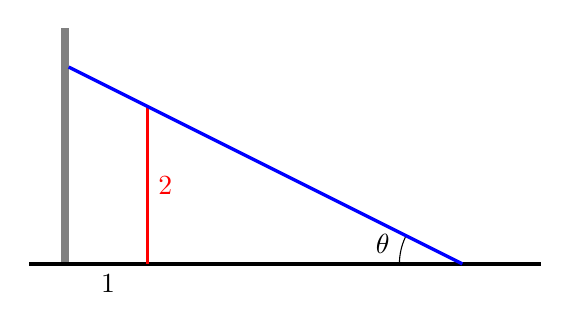
\begin{tikzpicture}
\fill[gray] (0,0) rectangle (-0.1,3);
\draw[very thick] (-0.5,0) -- (0.5,0) node[below] {1} -- (6,0);
\draw[very thick,red] (1,0) -- (1,1) node[right] {2} -- (1,2);
\draw[very thick,blue] (0,2.5) -- (5,0);
\draw (4.2, 0) arc(180:155:0.8);
\draw (4.2,0.25) node[left] {$\theta$};
\end{tikzpicture}
\end{flushright}
\hfill  \url{https://youtu.be/HdgZP3sfwuI} 
\hrule 


\item Simplify $\dfrac{1+ \cot^2(x)}{\csc^2(x) - 1}$. 
\vfill 
\hfill  \url{https://youtu.be/Z2buWFvEE7Y} 
\hrule 


\item Use the graph below to find the indicated limits. 
\begin{center}
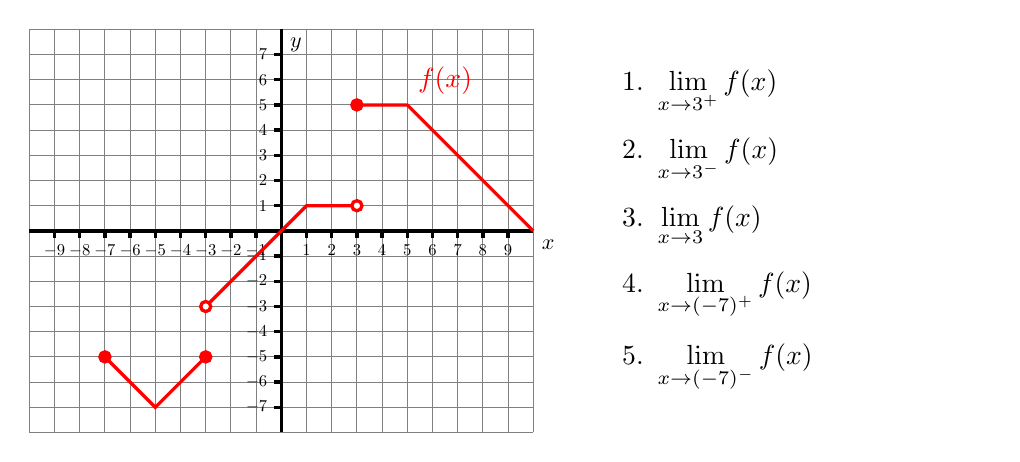
\begin{tikzpicture}[scale=0.32]
\draw[gray] (-10,-8) grid (10,8);
\draw[very thick] (-10,0) -- (10,0) node[below right,scale=0.8] {$x$};
\draw[very thick] (0,-8) -- (0,8) node[below right,scale=0.8] {$y$};
\foreach \x in {1,...,9} {
    \draw[very thick] (\x,0) -- (\x,-0.3) node[below,scale=0.6] {\x};
    \draw[very thick] (-\x,0) -- (-\x,-0.3) node[below,scale=0.6] {$-\x$};
}
\foreach \y in {1,...,7} {
    \draw[very thick] (0,\y) -- (-0.3,\y) node[left,scale=0.6] {\y};
    \draw[very thick] (0,-\y) -- (-0.3,-\y) node[left,scale=0.6] {$-\y$};
}
\draw[very thick, red] (-7,-5) -- (-5,-7) -- (-3,-5);
\draw[very thick, red] (-3,-3) -- (1,1) -- (3,1);
\draw[very thick, red] (3,5) -- (5,5) node[above right] {$f(x)$} -- (10,0);
\filldraw[very thick,draw=red,fill=white] (-3,-3) circle (0.2);
\filldraw[very thick,draw=red,fill=white] (3,1) circle (0.2);
\filldraw[very thick,draw=red,fill=red] (-7,-5) circle (0.2);
\filldraw[very thick,draw=red,fill=red] (-3,-5) circle (0.2);
\filldraw[very thick,draw=red,fill=red] (3,5) circle (0.2);

\draw (20,0) node {\begin{minipage}{5cm}
\begin{enumerate} 
\item $\ds \lim_{x \rightarrow 3^+} f(x)$
\item $\ds \lim_{x \rightarrow 3^-} f(x)$
\item $\ds \lim_{x \rightarrow 3} f(x)$
\item $\ds \lim_{x \rightarrow (-7)^+} f(x)$
\item $\ds \lim_{x \rightarrow (-7)^-} f(x)$
\end{enumerate}
\end{minipage} };

\end{tikzpicture}
\end{center}
\hfill  \url{https://youtu.be/qxhxp9IIEVo} 
\hrule 

\newpage

\item Find $\ds \lim_{x \rightarrow -1} \left( \frac{2x+2}{x+1} \right)$. 
\vfill 
\hfill  \url{https://youtu.be/GGQngIp0YGI} 
\hrule 

\item Let $g$ and $h$ be the functions in the graphs shown below. If $f(x) = g(x) h(x)$, then find $f'(4)$.
\begin{center}
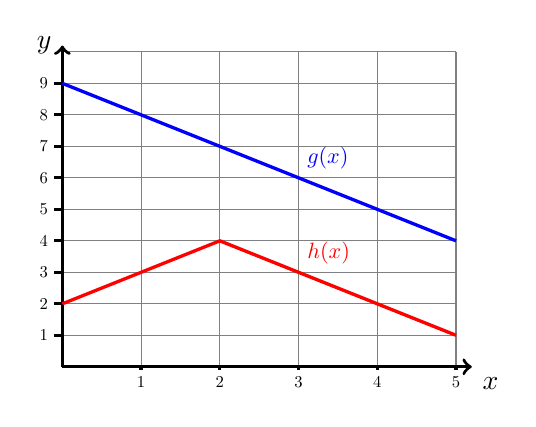
\begin{tikzpicture}
\begin{scope}[yscale = 0.4]
\draw[gray] (0,0) grid (5,10);
\draw[very thick,->] (0,0) -- (0,10.2) node[left,scale=1.0] {$y$};
\draw[very thick,->] (0,0) -- (5.2,0) node[below right,scale=1.0] {$x$};
\draw[very thick,blue] (0,9) -- (3,6) node[above right,scale=0.8] {$g(x)$} -- (5,4);
\draw[very thick,red] (0,2) -- (2,4) -- (3,3) node[above right,scale=0.8] {$h(x)$} -- (5,1);
\foreach \y in {1,...,9} {
  \draw[very thick] (0,\y) -- (-0.1,\y) node[left, scale=0.6] {\y};
}
\foreach \x in {1,...,5} {
  \draw[very thick] (\x,0) -- (\x, -0.1) node[below,scale=0.6] {\x};
}
\end{scope}

\end{tikzpicture}
\end{center}
\hfill  \url{https://youtu.be/1cHPPlmIzk0} 
\hrule 


\item Find the derivative of $f(x) = \dfrac{x^2}{\cos x}$. 
\vfill 
\hfill  \url{https://youtu.be/WqzY3xibFL8} 
\hrule 

\item Draw a rough sketch of the graph of the derivative of the function shown in the graph below. 
\begin{flushright}
\begin{tikzpicture}[xscale=0.7,yscale=0.7]
\draw[thick,<->] (-4.8,0) -- (2.8,0) node[right] {$x$};
\draw[thick,<->] (0,-2.8) -- (0,2.8) node[left] {$y$};
\foreach \x in {1,2} {
  \draw (\x,0.1) -- (\x,-0.1) node[below,scale=0.6] {\x};
}
\foreach \x in {-1,-2,-3,-4} {
  \draw (\x,0.1) -- (\x,-0.1) node[below,scale=0.6] {\x};
}
\foreach \y in {1,2} {
  \draw (0.1,\y) -- (-0.1,\y) node[left,scale=0.6] {\y};
  \draw (0.1,-\y) -- (-0.1,-\y) node[left,scale=0.6] {-\y};
}
\draw[very thick,color=blue, <->] plot[domain=-3.3:1.5,samples=400] function {(x**3 + 3*x**2-4)/3} node[right] {$f(x)$};
\end{tikzpicture}
\end{flushright}
\hfill \url{https://youtu.be/Kz_reJgi_Rg}
\hrule

\end{enumerate}
\end{document}



\item As you go deeper and deeper in the ocean, the pressure increases linearly.  At the surface, pressure is 1 atmosphere (ATM). For every 10 meters underwater, pressure increases by 1 additional ATM.
\begin{parts}
\part Find a formula for pressure (P) as a function of depth underwater (d)
\vfill

\part Draw and label a graph of pressure vs. depth.
\begin{center}
\begin{tikzpicture}[scale=1]
\draw[very thick,<->] (-0.3,0) -- (5.3,0) node[below] {$d$};
\draw[very thick,<->] (0,-0.3) -- (0,4.3) node[left] {$P$};
\end{tikzpicture}
\end{center}

\part What is the derivative of the pressure function?  Your answer should be a number.Explain what this number represents and what units are used to measure it.
\vfill
\vfill
\end{parts}

\question[10] A rock thrown up in the air has height $h(t) = 8t - 16t^2 + 4$ measured in feet at time $t$ seconds.
\begin{parts}
\part Find a formula for the velocity of the rock as a function of time. 
\vfill

\part Find a formula for the acceleration of the rock.    
\vfill

\end{parts}
\newpage
\question[8] The graph of a function $g(x)$ is shown below.  The slope of the secant line that passes through points $P$ and $Q$ is represented by the difference quotient $\ds\frac{g(b) - g(a)}{b-a}$. 
\begin{flushright}
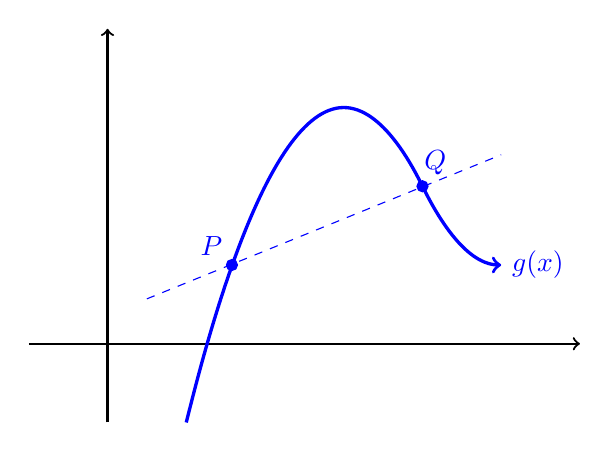
\begin{tikzpicture}
\draw[thick,->] (-1,0) -- (6,0);
\draw[thick,->] (0,-1) -- (0,4);
\draw[very thick, blue] (1,-1) parabola bend (3,3) (4,2);
\draw[very thick, blue,->] (4,2) parabola bend (5,1) (5,1) node[right] {$g(x)$};
\filldraw[blue] (4,2) circle (2pt) node[above=0.3cm, right=-0.1cm] {$Q$};
\filldraw[blue] (1.58,1) circle (2pt) node[above left] {$P$};
\draw[dashed, blue] (0.5,0.57) -- (5,2.4);
\end{tikzpicture}
\end{flushright}

\begin{parts}
\part Which part of the difference quotient represents the $x$-coordinate of $P$? \\
\part Which part of the difference quotient represents the $y$-coordinate of $P$? \\
\part Which part of the difference quotient represents the $x$-coordinate of $Q$? \\
\part Which part of the difference quotient represents the $y$-coordinate of $Q$? \\
\end{parts} 

\vspace*{0.25in}

\question[10] Use the limit definition of the derivative $\ds f'(x) = \lim_{h \rightarrow 0} \frac{f(x+h)-f(x)}{h}$ to find the derivative of $f(x) = \ds \frac{1}{2x}$.  
\vfill


\newpage
\question[20] Find the following derivatives using any valid method.  You don't have to simplify your answers.
\begin{parts}
\item $\ds \frac{d}{dx} \, 2x^6 - 5x^3 + 5x$
\vfill

\item $\ds \frac{d}{dx} \, \frac{\tan x}{\sin x}$
\vfill

\item $\ds \frac{d}{dt} \sqrt{t} (5-\sqrt{t})$
\vfill

\item $\ds \frac{d}{dr} \, \frac{4}{r^3}$
\vfill

\item $\ds \frac{d}{dx} \, \sec (4x)$
\vfill


\end{parts} 

\question[6] Suppose that $f$ and $g$ are functions such that $f(5) = 3$, $g(3) = -4$, $f'(5) = 2$, and $g'(3) = \frac{1}{2}$.  
\begin{parts}
\part Find $g(f(5))$.
\vfill

\part Find the derivative of $g(f(x))$ at $x=5$.  
\vfill
\end{parts} 


\newpage

\question[10] Use the axes below to sketch a graph of the parabola 
$$y=-x^2+4x-3.$$ 
Include the coordinates of the vertex and the roots of the parabola in your graph.  

\begin{center}
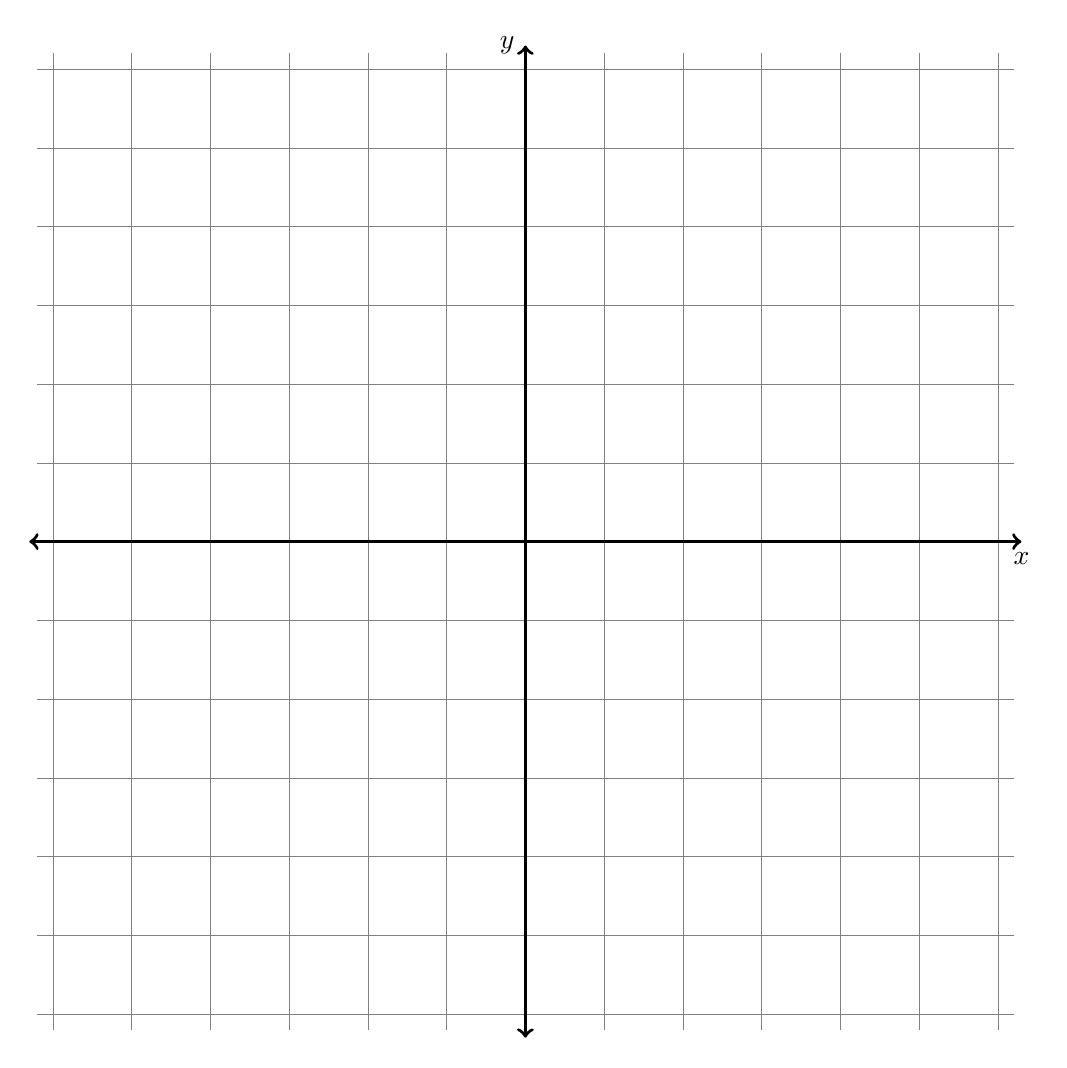
\begin{tikzpicture}
\draw[black!50,very thin] (-6.2,-6.2) grid (6.2,6.2);
\draw[very thick,<->] (-6.3,0) -- (6.3,0) node[below] {$x$};
\draw[very thick,<->] (0,-6.3) -- (0,6.3) node[left] {$y$};
\end{tikzpicture}
\end{center} 

\question[8] Find a formula for the tangent line to the parabola above at the point $(0,-3)$.  Once you find this tangent line, add its graph to the graph above.  
\vfill

\newpage

\question[16] The function $f(x) = \sin(x^2)$ has the graph shown below.  
\begin{center}
\begin{tikzpicture}[scale=2]
\draw[black!50,very thin] (-3.2,-1.7) grid (3.2,1.7);
\draw[very thick,<->] (-3.3,0) -- (3.3,0) node[below] {$x$};
\draw[very thick,<->] (0,-1.8) -- (0,1.8) node[left] {$y$};
%\draw[very thick,color=blue] plot[domain=-3.2:3.2,samples=400] function {sin(x**2)};
\end{tikzpicture}
\end{center} 

\begin{parts}
\part Is this function even, odd, or neither?  
\vfill

\part Use the chain rule to find $f'(x)$.  
\vfill
\vfill

\part Find the $x$-coordinates of all the points where $f(x)$ has a horizontal tangent.  
\vfill
\vfill

\end{parts}
\end{questions}


\input{formulas.tex}
\end{document}














